\section{Case-Studies}
In this section we present two case-studies in simulating the \textit{Prisoners Dilemma} and \textit{Heroes \& Cowards} games for discussing the effect of using different update-strategies. As already emphasised in this section, both are of different nature. The first one is a discrete game, played at discrete time-steps. The second one is a continuous game where each agent is continuously playing. This has profound implications on the simulation results as will is shown below. We implemented the simulations for all strategies except the \textit{actor strategy} in Java and the simulations for the \textit{actor strategy} in Haskell and in Scala with the Actor-Library.

\begin{figure*}
\begin{center}

	\begin{tabular}{c c}
		\textbf{Prisoners Dilemma} & \textbf{Heroes \& Cowards} \\ 

		\begin{subfigure}[b]{0.4\textwidth}
			\centering
			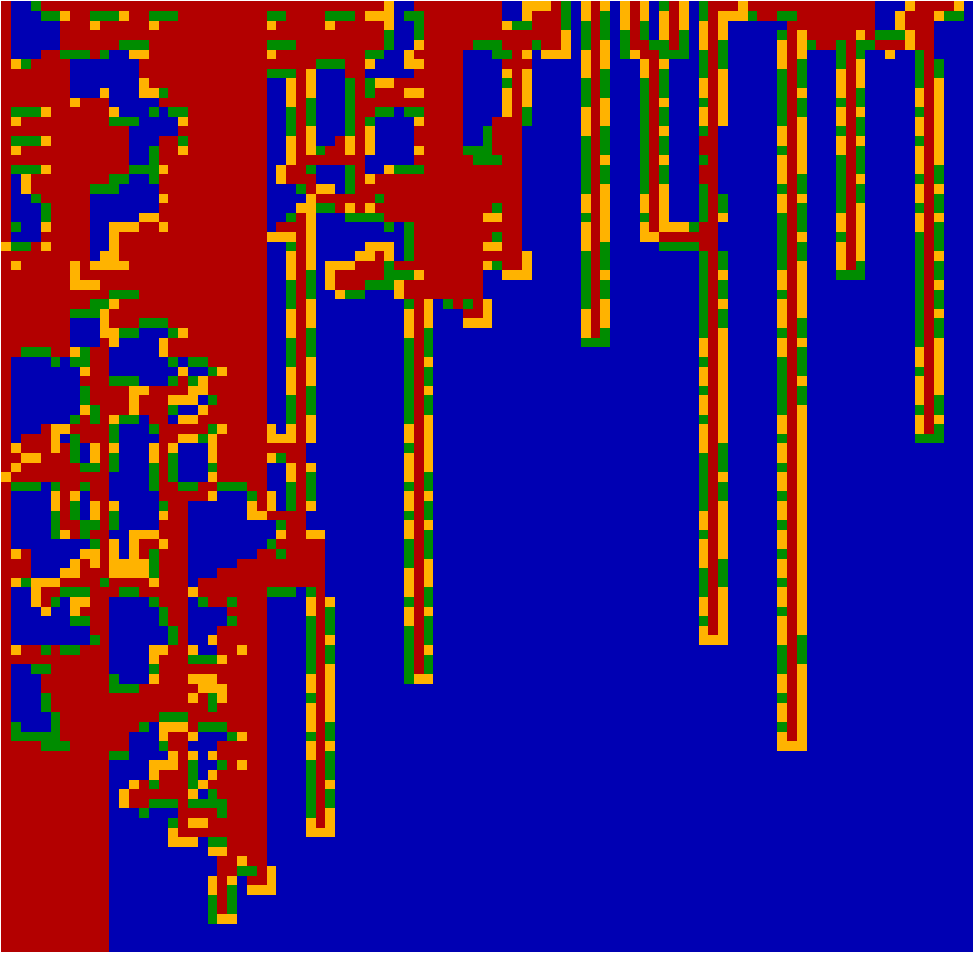
\includegraphics[width=.7\textwidth, angle=0]{./fig/seq_QUEUED_SG_436steps_java.png}
			\caption{sequential queued}
			\label{fig:pd_seq}
		\end{subfigure}
    	&
		\begin{subfigure}[b]{0.4\textwidth}
			\centering
			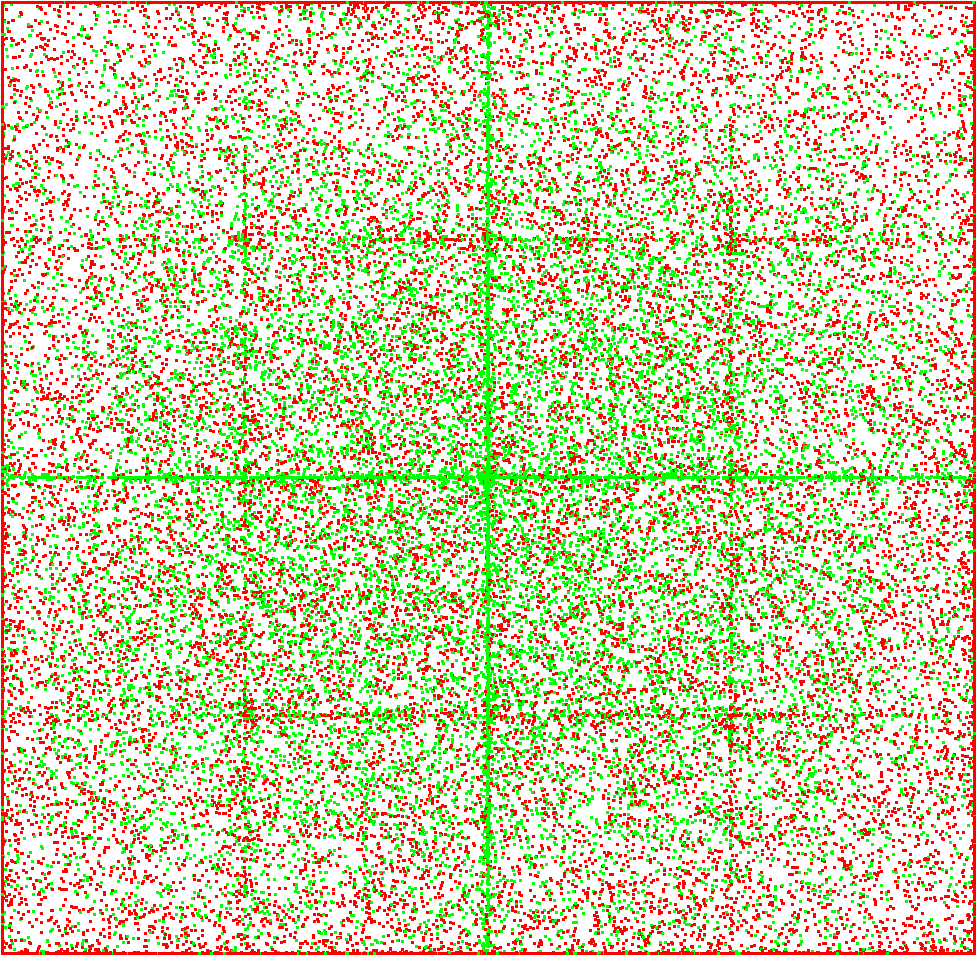
\includegraphics[width=.7\textwidth, angle=0]{./fig/seq_HAC_100_000_500steps_java.png}
			\caption{sequential}
			\label{fig:hac_seq}
		\end{subfigure}
    	\\
    	
		
		\begin{subfigure}[b]{0.4\textwidth}
			\centering
			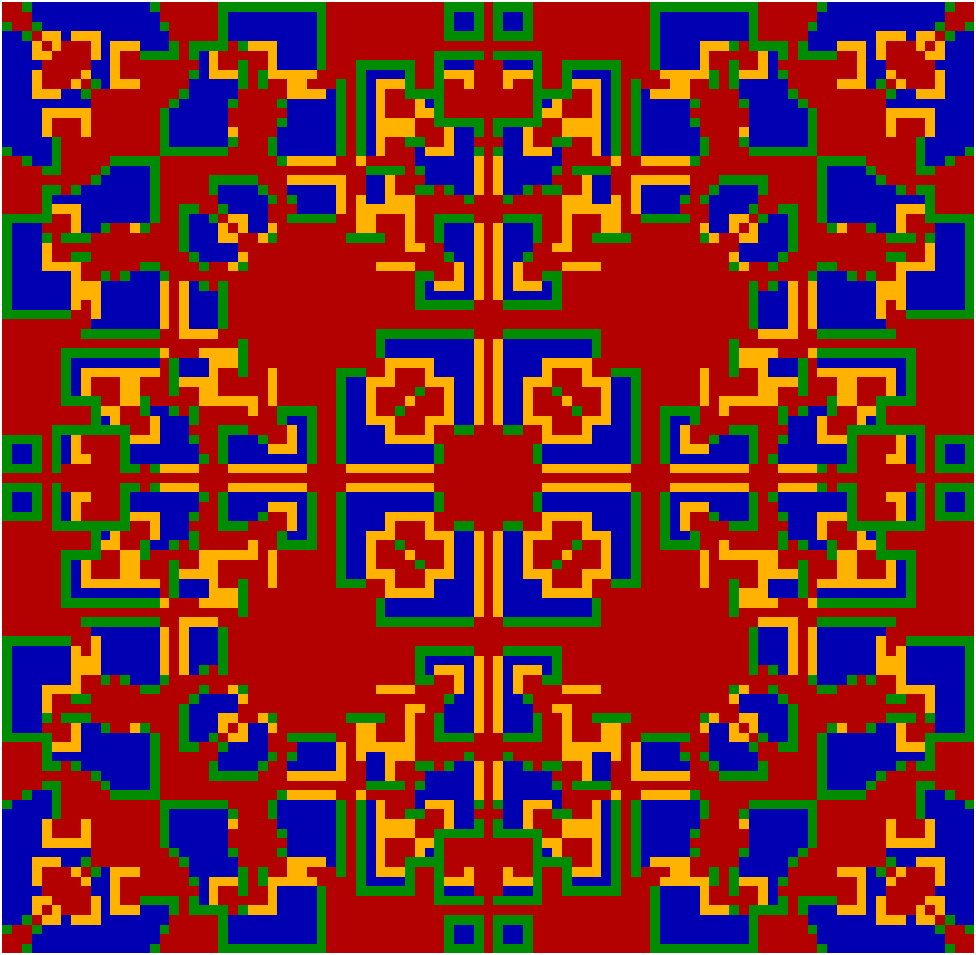
\includegraphics[width=.7\textwidth, angle=0]{./fig/par_SG_436steps_java.png}
			\caption{parallel}
			\label{fig:pd_par}
		\end{subfigure}
    	&
		\begin{subfigure}[b]{0.4\textwidth}
			\centering
			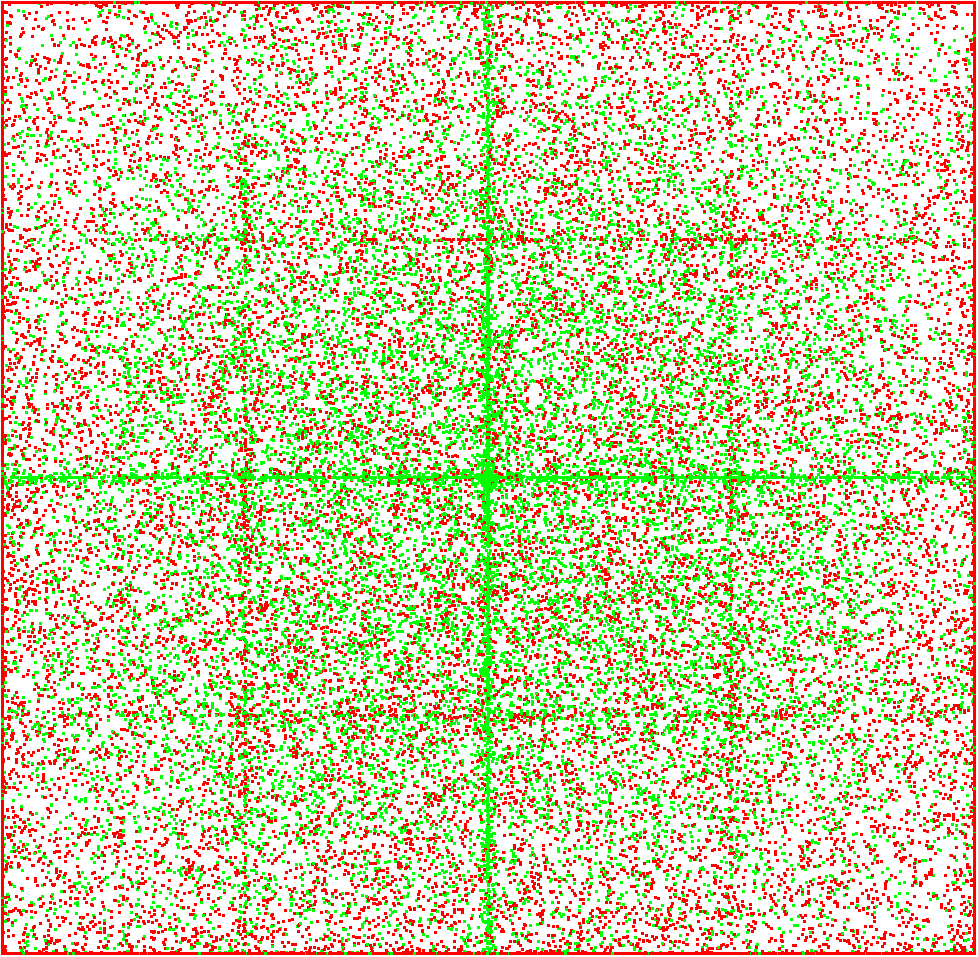
\includegraphics[width=.7\textwidth, angle=0]{./fig/par_HAC_100_000_500steps_java.png}
			\caption{parallel}
			\label{fig:hac_par}
		\end{subfigure}
    	\\
		
		\begin{subfigure}[b]{0.4\textwidth}
			\centering
			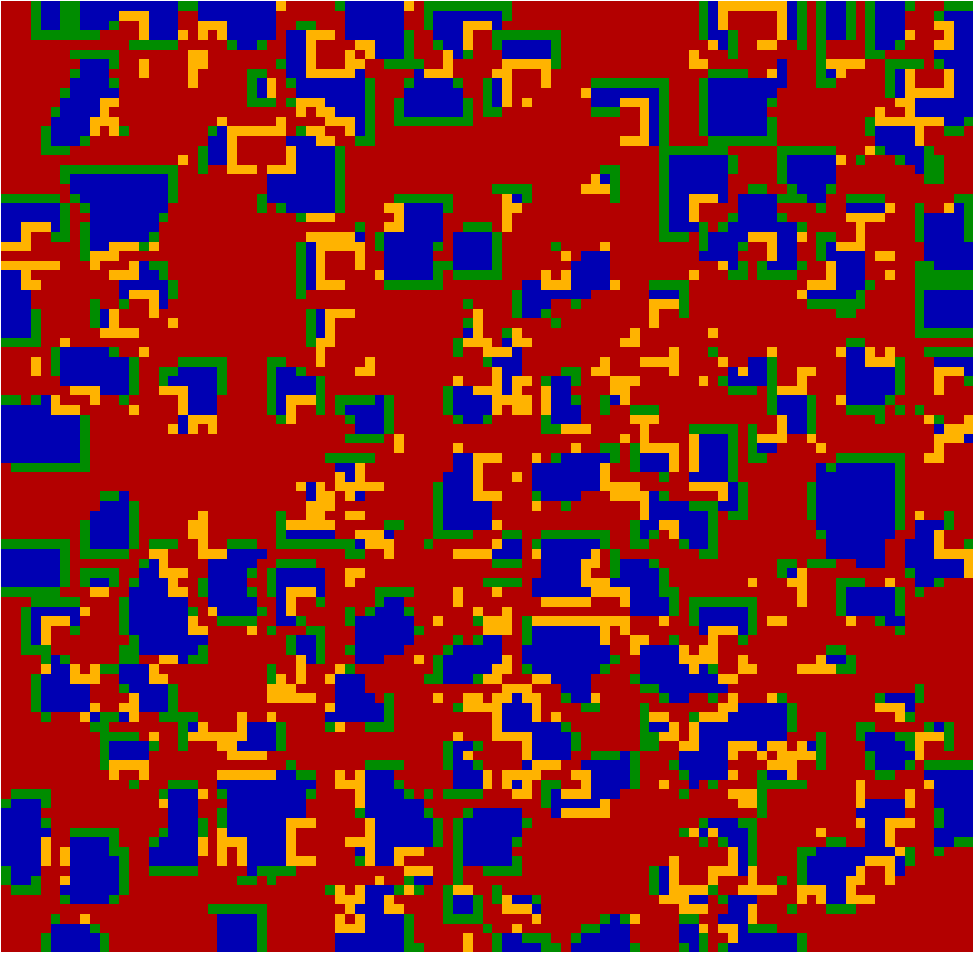
\includegraphics[width=.7\textwidth, angle=0]{./fig/con_SG_436steps_java.png}
			\caption{concurrent}
			\label{fig:pd_con}
		\end{subfigure}
    	&
		\begin{subfigure}[b]{0.4\textwidth}
			\centering
			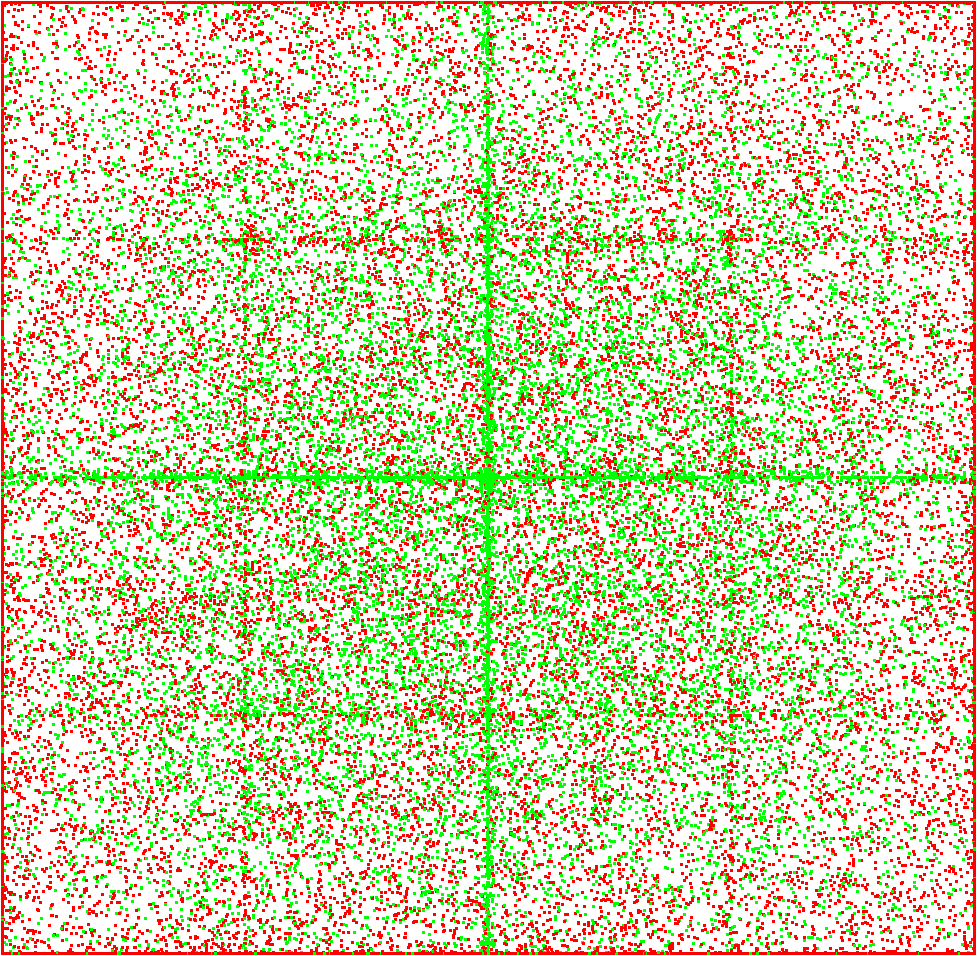
\includegraphics[width=.7\textwidth, angle=0]{./fig/con_HAC_100_000_500steps_java.png}
			\caption{concurrent}
			\label{fig:hac_con}
		\end{subfigure}
    	\\ 
		
		\begin{subfigure}[b]{0.4\textwidth}
			\centering
			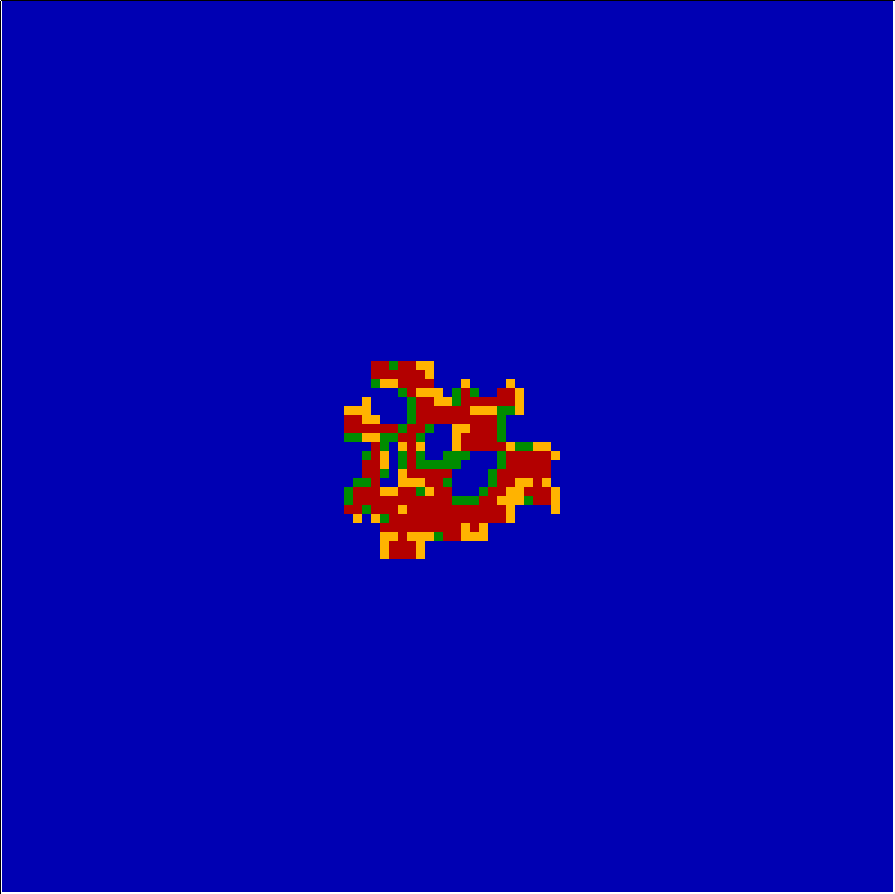
\includegraphics[width=.7\textwidth, angle=0]{./fig/act_SG_scala.png}
			\caption{actor}
			\label{fig:pd_act}
		\end{subfigure}
    	& 
		\begin{subfigure}[b]{0.4\textwidth}
			\centering
			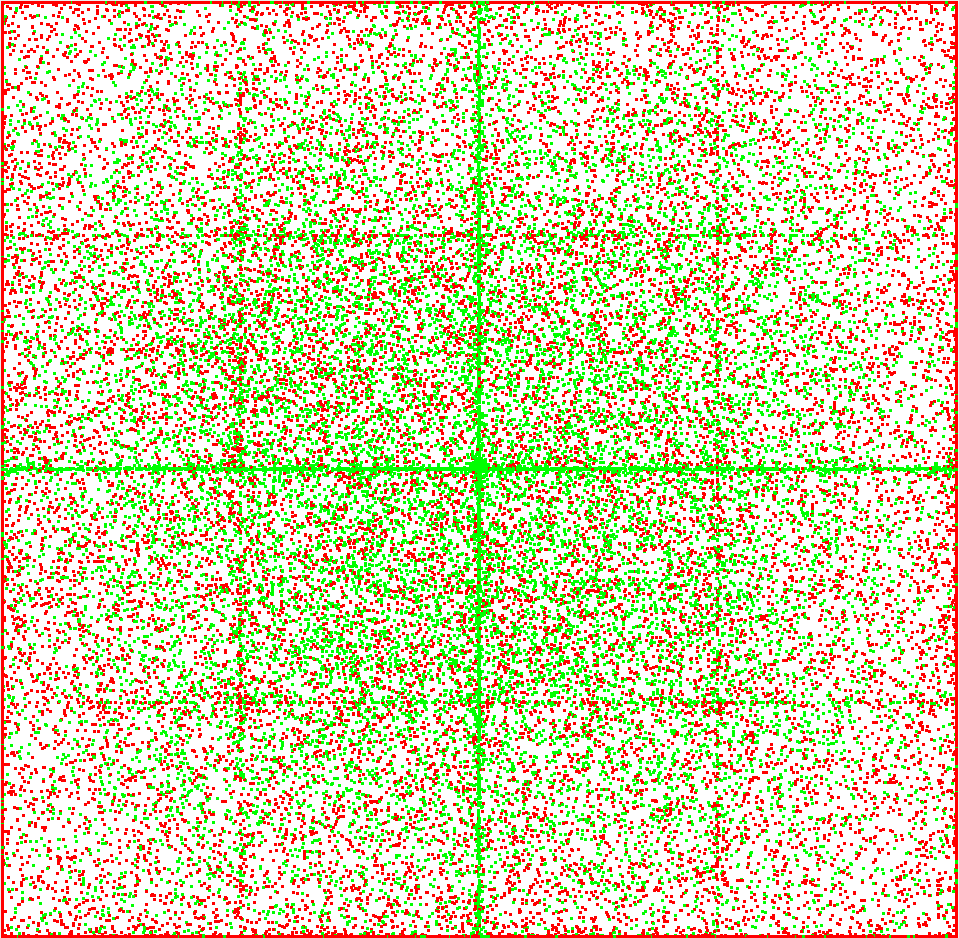
\includegraphics[width=.7\textwidth, angle=0]{./fig/act_HAC_100_000_500steps_scala.png}
			\caption{actor}
			\label{fig:hac_act}
		\end{subfigure}

	\end{tabular}
	
	\caption{\small Effect on results simulating the Prisoners Dilemma and Heroes \& Cowards with all four update-strategies.} 
	\label{fig:results}
	
\end{center}
\end{figure*}

\subsection{Prisoners Dilemma}
\paragraph{The agent-based model}
Our agent-based model of this game works as follows: at the start of the simulation each agent sends its state to all its neighbours which allows to incrementally calculate the local payoff. If all neighbours states have been received then the agent will send its local payoff to all neighbours which allows to compare all payoffs in its neighbourhood and calculate the best. When all neighbours local payoff have been received the agent will adopt the role of the highest payoff and sends its new state to all its neighbours, creating a circle. 

Care must be taken to ensure that the update-strategies are comparable because when implementing a model in an update-strategy it is necessary to both map the model to the strategy and try to stick to the same specification - if the implementation of the model differs fundamentally across the update-strategies it is not possible to compare the solutions. So we put great emphasis and care keeping all four implementations of the model the same just with a different update-strategy running behind the scenes which guarantees comparability.

\paragraph{Results}
The results as seen in the left column of Figure \ref{fig:results} were created with the same configuration as reported in \cite{nowak_evolutionary_1992}. When comparing the pictures with the one from the reference seen in Figure \ref{fig:sync_patterns} the only update-strategy which is able to reproduce the matching result is the \textit{parallel strategy} - all the others clearly fail to reproduce the pattern. From this we can tell that only the \textit{parallel strategy} is suitable to simulate this model. 

To reproduce the pattern of Figure \ref{fig:sync_patterns} the simulation needs to be split into two global steps which must happen after each other: first calculating the sum of all payoffs for every agent and then selecting the role of the highest payoff within the neighbourhood. This two-step approach results in the need for twice as many steps to arrive at the matching pattern when using \textit{queued} messaging as is the case in the \textit{parallel, concurrent} and \textit{actor strategy}.

For the \textit{sequential strategy} one must further differentiate between \textit{immediate} and \textit{queued} messaging. We presented the results using the \textit{queued} version, which has the same implementation of the model as the others. When one is accepting to change the implementation slightly, then the \textit{immediate} version is able to arrive at the pattern after 217 steps with a slightly different model-implementation: because immediate messaging transfers the thread of control to the receiving agent that agent can reply within this same step. This implies that we can calculate a full game-round (both steps) within one global time-step by a slight change in the model-implementation: an agent sends its current state in every time-step to all its neighbours.

The reason why the other strategies fail to reproduce the pattern is due to the non-parallel and unsynchronized way that information spreads through the grid. In the \textit{sequential strategy} the agents further ahead in the queue play the game earlier and influence the neighbourhood so agents which play the game later find already messages from earlier agents in their queue thus acting differently based upon these informations. Also agents will send messages to itself which will be processed in the same time-step. In the \textit{concurrent} and \textit{actor strategy} the agents run in parallel but changes are visible immediately and concurrently, leading to the same non-structural patterns as in the \textit{sequential} one. Although agents don't change unless all their neighbours have answered, this does not guarantee a synchronized update of all agents because every agent has a different neighbourhood which is reflexive but not transitive. If agent \textit{a} is agents \textit{b} neighbour and agent \textit{c} is agent \textit{b} neighbour this does not imply that agent \textit{c} is agent \textit{a} neighbour as well. This allows the spreading of changes throughout the neighbourhood, resulting in a breaking down of the pattern.
This is not the case in the \textit{parallel strategy}  where all agents play the game at the same time based on the frozen state of the previous step, leading to a synchronized update as required by the model. Note that the \textit{concurrent} and \textit{actor strategy} produce different results on every run due to the inherent non-deterministic event-ordering introduce by concurrency.


\subsection{Heroes \& Cowards}
\paragraph{The agent-based model}
Our agent-based model of this game works as follows: in each time-step an agent asks its friend and enemy for their positions which will answer with a corresponding message containing their current positions. The agent will have its own local information about the position of its friend and enemy and will calculate its move in every step based on this local information.

\paragraph{Results}
The results as seen in the right column of Figure \ref{fig:results} were created with 100.000 agents where 25\% of them are heroes running for 500 steps. Although the individual agent-positions of runs with the same configuration differ between update-strategies the cross-patterns are forming in all four update-strategies. For the patterns to emerge it is important to have significant more cowards than heroes and to have agents in the tens of thousands - we went for 100.000 because then the patterns are really prominent. The patterns form because the heroes try to stay halfway between their friend and enemy: with this high number of cowards it is very likely that heroes end up with two cowards - the cowards will push towards the border as they try to escape leaving the hero in between. We can conclude that the \textit{Heroes \& Cowards} model seems to be robust to the selection of its update-strategy and that its emergent property - the formation of the cross - is stable under differing strategies.